% Edit only the text between matching begin and end lines.
\documentclass[11pt,a4paper]{article}
% Shared preamble for TMUA question papers. Local edits here are overwritten.

% Reproducible PDFs: no timestamps, no trailer id, no build-path details.
\ifdefined\pdfsuppressptexinfo
  \pdfsuppressptexinfo=-1
  \pdfinfoomitdate=1
  \pdftrailerid{}
\fi

\usepackage{graphicx}
\usepackage{mathtools}
\usepackage{amssymb}
\usepackage{amsmath}
\usepackage{amsthm}
\usepackage{enumitem}
\usepackage{microtype}
\usepackage[table]{xcolor}
\usepackage{array}
\usepackage{booktabs}
\usepackage{tabularx}
\usepackage{longtable}
\usepackage{ragged2e}
\usepackage{fancyhdr}
\usepackage{etoolbox}
\usepackage[
  a4paper,
  left=0.8in,
  right=1in,
  top=1in,
  bottom=0.5in,
  headheight=14pt,
  headsep=0.4in
]{geometry}

\usepackage{pgfplots}
\pgfplotsset{compat=1.18}
\usepgfplotslibrary{fillbetween, polar}
\usetikzlibrary{calc, positioning}
\usetikzlibrary{angles, quotes}
\usetikzlibrary{arrows.meta}
\usetikzlibrary{decorations.pathreplacing, decorations.markings}
\usetikzlibrary{patterns}
\usetikzlibrary{intersections}

\usepackage{tocloft}
\usepackage[hidelinks]{hyperref}
\hypersetup{pdfauthor={danieljsmith.org}, pdfcreator={}, pdfsubject={}, pdfkeywords={}}
\urlstyle{same}
\tocloftpagestyle{djspaper}
\setlength{\cftbeforesubsecskip}{2pt}
\setlength{\cftsubsecindent}{1.5em}
\setlength{\cftsubsecnumwidth}{0pt}
\renewcommand{\cftsubsecfont}{\small\color{black}}
\renewcommand{\cftsubsecpagefont}{\small\color{black}}
\renewcommand{\cftsubsecleader}{\hfill}

% \djsPaperSetup{<PDF title>}{<header label>}, called once after this file.
\newcommand{\djsHeaderLabel}{}
\newcommand{\djsPaperSetup}[2]{%
  \hypersetup{pdftitle={#1}}%
  \renewcommand{\djsHeaderLabel}{#2}}

% \djsTitleSetup{<booklet>}{<title>}{<paper name>}{<questions>}{<minutes>},
% called once after the setup line, sets the title block that opens the
% contents page and the answer key: TMUA and the booklet in spaced burgundy
% capitals, the title, a hairline led by a short scarlet rule, then the
% paper's name with the question count and, when given, the time allowed.
% Its colours are the site's accent, rule and muted text colours.
\definecolor{scarlet}{RGB}{205, 40, 75}
\definecolor{djsBurgundy}{RGB}{118, 59, 67}
\definecolor{djsHairline}{RGB}{216, 213, 205}
\definecolor{djsSlash}{RGB}{170, 166, 158}
\definecolor{djsMuted}{RGB}{96, 101, 106}
\makeatletter
\newcommand{\djs@booklet}{}
\newcommand{\djs@title}{}
\newcommand{\djs@papername}{}
\newcommand{\djs@details}{}
\newcommand{\djs@caps}[1]{\textls[180]{\MakeUppercase{#1}}}
\newcommand{\djs@dot}{\hspace{0.45em}\textperiodcentered\hspace{0.45em}}
\newcommand{\djsTitleSetup}[5]{%
  \renewcommand{\djs@booklet}{#1}%
  \renewcommand{\djs@title}{#2}%
  \renewcommand{\djs@papername}{#3}%
  \renewcommand{\djs@details}{%
    #4~question\ifnum#4=1 \else s\fi
    \ifblank{#5}{}{\djs@dot#5~minutes}}}
\newcommand{\djsContentsTitle}{%
  {\raggedright\color{djsBurgundy}\footnotesize\bfseries
    \djs@caps{TMUA}{\color{djsSlash}\hspace{0.55em}/\hspace{0.55em}}%
    \djs@caps{\djs@booklet}\par}%
  \vspace{7pt}%
  {\raggedright\fontsize{24.88}{28}\selectfont\djs@title\par}%
  \vspace{9pt}%
  \noindent\makebox[0pt][l]{\color{djsHairline}\rule[0.9pt]{\linewidth}{0.6pt}}%
  {\color{scarlet}\rule{3.5cm}{2.2pt}}\par
  \vspace{5pt}%
  {\small\color{djsMuted}\djs@papername\hfill\djs@details\par}%
  \vspace{8pt}}
\makeatother

\setlength{\parindent}{0pt}
\fancypagestyle{djspaper}{%
  \fancyhead{}%
  \fancyfoot{}%
  \renewcommand{\headrulewidth}{0.9pt}%
  \fancyhead[L]{\djsHeaderLabel}%
  \fancyhead[R]{\href{https://danieljsmith.org/?utm_source=pdf&utm_campaign=tmua&utm_content=questions}{danieljsmith.org}}%
}
\pagestyle{djspaper}

% \djsLastUpdated{<date>}, called once after the setup line: one line
% at the foot of the first page only, left-aligned under the left header at
% the 0.8in left margin. It is drawn over the page rather than set as a
% footer, so no page style changes.
\newcommand{\djsLastUpdated}[1]{%
  \AtBeginDocument{\AddToHookNext{shipout/foreground}{%
    \put(0.8in,-\dimexpr\paperheight-0.32in\relax){\makebox[0pt][l]{%
      \footnotesize Last updated #1}}}}}

\newcolumntype{Y}{>{\RaggedRight\arraybackslash}X}

% Topic labels: a subtle line above each question and a suffix on its
% contents entry. The bookmark form is spelled out separately, because a PDF
% bookmark is plain text and would otherwise keep the colour name.
\newcommand{\djsTocTopic}[1]{%
  \ifblank{#1}{}{%
    \texorpdfstring
      {\hspace{0.9em}{\footnotesize\itshape\color{black!45}#1}}
      { \textendash\ #1}}}
\newcommand{\djsTopicLine}[1]{%
  \ifblank{#1}{}{%
    {\raggedleft\footnotesize\itshape\color{black!45}#1\par}%
    \vspace{-0.6\baselineskip}}}

\newcommand{\questionitem}[1][]{%
  \item\phantomsection
  \addcontentsline{toc}{subsection}{%
    Question \number\value{enumi}\protect\djsTocTopic{#1}}%
}
\renewcommand{\contentsname}{Questions}
\newcommand{\djsFrontMatter}{%
  \vspace*{6pt}%
  \djsContentsTitle
  \vspace{14pt}%
  \tableofcontents
  \newpage
}

\djsPaperSetup{TMUA Set C Paper 2}{TMUA Set C - Paper 2}
\djsLastUpdated{2 October 2026}
\begin{document}
\thispagestyle{djspaper}
\djsFrontMatter
\thispagestyle{djspaper}
\vspace*{8pt}
\djsTopicLine{Trigonometry}
\begin{enumerate}[label=\textbf{\arabic*.},leftmargin=*,itemsep=0pt,start=1]
\questionitem[Trigonometry]
% begin q000726 stem
A triangle $ABC$ has $\angle BAC=30^\circ$, $BC=2$ and $AC=2\sqrt{3}$. 

Two different triangles satisfy these conditions. 

What is the sum of their areas?
% end q000726 stem

\par\vspace*{12pt}
\begin{tabularx}{\linewidth}{@{}>{\bfseries}l Y@{}}
A &
% begin q000726 choice A
$\sqrt{3}$
% end q000726 choice A
\\[0.8em]
B &
% begin q000726 choice B
$2\sqrt{3}$
% end q000726 choice B
\\[0.8em]
C &
% begin q000726 choice C
$3\sqrt{3}$
% end q000726 choice C
\\[0.8em]
D &
% begin q000726 choice D
$4\sqrt{3}$
% end q000726 choice D
\\[0.8em]
E &
% begin q000726 choice E
$6\sqrt{3}$
% end q000726 choice E
\\
\end{tabularx}
\end{enumerate}
\clearpage
\thispagestyle{djspaper}
\vspace*{8pt}
\djsTopicLine{Logic}
\begin{enumerate}[label=\textbf{\arabic*.},leftmargin=*,itemsep=0pt,start=2]
\questionitem[Logic]
% begin q000121 stem
Let $f(x),\, g(x)$ and $h(x)$ be real functions and consider the statement \begin{equation}\tag{$\ast$} \text{If $x>0$ and $f(x)\le 0$ then $g(x)\neq 1$ or $h(x)\ge -1$}\\[5pt] \end{equation} Which of the following statements is the \textit{contrapositive} of ($\ast$)?
% end q000121 stem

\par\vspace*{12pt}
\begin{tabularx}{\linewidth}{@{}>{\bfseries}l Y@{}}
A &
% begin q000121 choice A
If $g(x) = 1$ and $h(x) < -1$ then $x \le 0$ or $f(x) > 0$
% end q000121 choice A
\\[0.8em]
B &
% begin q000121 choice B
If $g(x) = 1$ or $h(x) < -1$ then $x \le 0$ or $f(x) > 0$
% end q000121 choice B
\\[0.8em]
C &
% begin q000121 choice C
If $x \le 0$ or $f(x) > 0$ then $g(x) = 1$ and $h(x) < -1$
% end q000121 choice C
\\[0.8em]
D &
% begin q000121 choice D
If $g(x) \neq 1$ or $h(x) \ge -1$ then $x > 0$ and $f(x) \le 0$
% end q000121 choice D
\\[0.8em]
E &
% begin q000121 choice E
If $x > 0$ and $f(x) \le 0$ then $g(x) = 1$ and $h(x) < -1$
% end q000121 choice E
\\[0.8em]
F &
% begin q000121 choice F
If $g(x) = 1$ and $h(x) < -1$ then $x \le 0$ and $f(x) > 0$
% end q000121 choice F
\\
\end{tabularx}
\end{enumerate}
\clearpage
\thispagestyle{djspaper}
\vspace*{8pt}
\djsTopicLine{Logic}
\begin{enumerate}[label=\textbf{\arabic*.},leftmargin=*,itemsep=0pt,start=3]
\questionitem[Logic]
% begin q000723 stem
Consider the equation

\[
4^x - 3 \times 2^x + k = 0
\]

where $k$ is a real constant.

Which of the following statements is/are true?

\[
\begin{array}{@{}ll@{}}
\textbf{I} & \text{For the equation to have a real solution, it is necessary that } k < 0 \\[5pt]
\textbf{II} & \text{For the equation to have a real solution, it is sufficient that } k < 0 \\[5pt]
\textbf{III} & \text{For the equation to have two distinct real solutions, it is necessary and} \\
& \text{sufficient that } 0 < k < \dfrac{9}{4} \\[5pt]
\end{array}
\]
% end q000723 stem

\par\vspace*{12pt}
\begin{tabularx}{\linewidth}{@{}>{\bfseries}l Y@{}}
A &
% begin q000723 choice A
None of them
% end q000723 choice A
\\[0.8em]
B &
% begin q000723 choice B
I only
% end q000723 choice B
\\[0.8em]
C &
% begin q000723 choice C
II only
% end q000723 choice C
\\[0.8em]
D &
% begin q000723 choice D
III only
% end q000723 choice D
\\[0.8em]
E &
% begin q000723 choice E
I and II only
% end q000723 choice E
\\[0.8em]
F &
% begin q000723 choice F
I and III only
% end q000723 choice F
\\[0.8em]
G &
% begin q000723 choice G
II and III only
% end q000723 choice G
\\[0.8em]
H &
% begin q000723 choice H
I, II and III
% end q000723 choice H
\\
\end{tabularx}
\end{enumerate}
\clearpage
\thispagestyle{djspaper}
\vspace*{8pt}
\djsTopicLine{Logic}
\begin{enumerate}[label=\textbf{\arabic*.},leftmargin=*,itemsep=0pt,start=4]
\questionitem[Logic]
% begin q000724 stem
An infinite geometric series
\[
a + ar + ar^2 + ar^3 + \cdots
\]
where $a \ne 0$, has sum to infinity $S$.

Which of the following statements is/are true?
\[
\begin{array}{@{}ll@{}}
\textbf{I} & S > a \textbf{ only if } r > 0 \\[5pt]
\textbf{II} & r > 0 \text{ is }\textbf{sufficient}\text{ for } S>a  \\[5pt]
\textbf{III} & a \text{ and } r \text{ being both positive or both negative is}\textbf{ necessary and sufficient} \text{ for } S > a
\end{array}
\]
% end q000724 stem

\par\vspace*{12pt}
\begin{tabularx}{\linewidth}{@{}>{\bfseries}l Y@{}}
A &
% begin q000724 choice A
None of them
% end q000724 choice A
\\[0.8em]
B &
% begin q000724 choice B
I only
% end q000724 choice B
\\[0.8em]
C &
% begin q000724 choice C
II only
% end q000724 choice C
\\[0.8em]
D &
% begin q000724 choice D
III only
% end q000724 choice D
\\[0.8em]
E &
% begin q000724 choice E
I and II only
% end q000724 choice E
\\[0.8em]
F &
% begin q000724 choice F
I and III only
% end q000724 choice F
\\[0.8em]
G &
% begin q000724 choice G
II and III only
% end q000724 choice G
\\[0.8em]
H &
% begin q000724 choice H
I, II and III
% end q000724 choice H
\\
\end{tabularx}
\end{enumerate}
\clearpage
\thispagestyle{djspaper}
\vspace*{8pt}
\djsTopicLine{Proof \& Error Analysis}
\begin{enumerate}[label=\textbf{\arabic*.},leftmargin=*,itemsep=0pt,start=5]
\questionitem[Proof \& Error Analysis]
% begin q000617 stem
A student proves that $\sqrt{2}$ is irrational, using proof by contradiction. The proof uses the following five statements, presented here in a scrambled order. \\

\begin{tabular}{@{}r@{\hspace{0.6em}}p{\dimexpr\linewidth-2.6em\relax}@{}}
(1) &
Since $p$ is even, write $p = 2k$ for some positive integer $k$; substituting into $p^2 = 2q^2$ gives $4k^2 = 2q^2$, so $q^2 = 2k^2$, and therefore $q$ is even.
\\[0.8em]

(2) &
Suppose, for contradiction, that $\sqrt{2}$ is rational, so $\sqrt{2} = \dfrac{p}{q}$ for some positive integers $p$ and $q$ with no common factor greater than $1$.
\\[0.8em]

(3) &
This means $p$ and $q$ share the common factor $2$, contradicting the assumption that $p$ and $q$ have no common factor greater than $1$.
\\[0.8em]

(4) &
Squaring both sides of $\sqrt{2} = \dfrac{p}{q}$ gives $p^2 = 2q^2$, so $p^2$ is even, and therefore $p$ is even.
\\[0.8em]

(5) &
Therefore the original assumption is false, and $\sqrt{2}$ is irrational.\\[0.8em]
\end{tabular}

\medskip

Which ordering of the statements (1)--(5) gives a valid proof, with each statement following logically from those before it?
% end q000617 stem

\par\vspace*{12pt}
\begin{tabularx}{\linewidth}{@{}>{\bfseries}l Y@{}}
A &
% begin q000617 choice A
2, 4, 1, 3, 5
% end q000617 choice A
\\[0.8em]
B &
% begin q000617 choice B
2, 1, 4, 3, 5
% end q000617 choice B
\\[0.8em]
C &
% begin q000617 choice C
4, 2, 1, 3, 5
% end q000617 choice C
\\[0.8em]
D &
% begin q000617 choice D
2, 4, 3, 1, 5
% end q000617 choice D
\\[0.8em]
E &
% begin q000617 choice E
2, 4, 1, 5, 3
% end q000617 choice E
\\[0.8em]
F &
% begin q000617 choice F
2, 3, 4, 1, 5
% end q000617 choice F
\\[0.8em]
G &
% begin q000617 choice G
2, 4, 3, 5, 1
% end q000617 choice G
\\[0.8em]
H &
% begin q000617 choice H
No ordering of the statements gives a valid proof.
% end q000617 choice H
\\
\end{tabularx}
\end{enumerate}
\clearpage
\thispagestyle{djspaper}
\vspace*{8pt}
\djsTopicLine{Sequences \& Series}
\begin{enumerate}[label=\textbf{\arabic*.},leftmargin=*,itemsep=0pt,start=6]
\questionitem[Sequences \& Series]
% begin q000768 stem
A geometric progression has a real first term and a real common ratio.

The sum of the first three terms is $14$, and the sum of the first six terms is $126$.

What is the sum of the first nine terms?
% end q000768 stem

\par\vspace*{12pt}
\begin{tabularx}{\linewidth}{@{}>{\bfseries}l Y@{}}
A &
% begin q000768 choice A
$98$
% end q000768 choice A
\\[0.8em]
B &
% begin q000768 choice B
$252$
% end q000768 choice B
\\[0.8em]
C &
% begin q000768 choice C
$511$
% end q000768 choice C
\\[0.8em]
D &
% begin q000768 choice D
$1022$
% end q000768 choice D
\\[0.8em]
E &
% begin q000768 choice E
$1092$
% end q000768 choice E
\\[0.8em]
F &
% begin q000768 choice F
$1134$
% end q000768 choice F
\\
\end{tabularx}
\end{enumerate}
\clearpage
\thispagestyle{djspaper}
\vspace*{8pt}
\djsTopicLine{Logic}
\begin{enumerate}[label=\textbf{\arabic*.},leftmargin=*,itemsep=0pt,start=7]
\questionitem[Logic]
% begin q000685 stem
Let $\theta$ be a real number with $0 < \theta < 2\pi$.

Consider the following three statements about the inequality \(\sin\theta + \cos\theta > 1\)

\[
\begin{array}{@{}l l@{}}
\textbf{I:} & \text{A necessary condition for the inequality to hold is that $\sin\theta\cos\theta > 0$} \\[5pt]
\textbf{II:} & \text{A sufficient condition for the inequality to hold is that $\sin\theta\cos\theta > 0$} \\[5pt]
\textbf{III:} &
\begin{aligned}[t]
&\text{A necessary and sufficient condition for the inequality to hold is that} \\
&\sin\theta\cos\theta > 0 \text{ and } \sin\theta + \cos\theta > 0 
\end{aligned}
\end{array}
\]

Which of the statements is/are true?
% end q000685 stem

\par\vspace*{12pt}
\begin{tabularx}{\linewidth}{@{}>{\bfseries}l Y@{}}
A &
% begin q000685 choice A
None of them
% end q000685 choice A
\\[0.8em]
B &
% begin q000685 choice B
I only
% end q000685 choice B
\\[0.8em]
C &
% begin q000685 choice C
II only
% end q000685 choice C
\\[0.8em]
D &
% begin q000685 choice D
III only
% end q000685 choice D
\\[0.8em]
E &
% begin q000685 choice E
I and II only
% end q000685 choice E
\\[0.8em]
F &
% begin q000685 choice F
I and III only
% end q000685 choice F
\\[0.8em]
G &
% begin q000685 choice G
II and III only
% end q000685 choice G
\\[0.8em]
H &
% begin q000685 choice H
I, II and III
% end q000685 choice H
\\
\end{tabularx}
\end{enumerate}
\clearpage
\thispagestyle{djspaper}
\vspace*{8pt}
\djsTopicLine{Geometry}
\begin{enumerate}[label=\textbf{\arabic*.},leftmargin=*,itemsep=0pt,start=8]
\questionitem[Geometry]
% begin q000649 stem
A solid cuboid has edges of length $1$ cm, $2$ cm and $3$ cm. 

An ant starts at one corner $S$ of the cuboid and crawls across the outside surfaces to the corner $F$ furthest from it. That is, the corner not sharing any face with the starting corner. 

The ant may cross any face but cannot pass through the inside of the cuboid. 

What is the shortest possible distance the ant travels?
% end q000649 stem

\begin{center}
% begin q000649 diagram
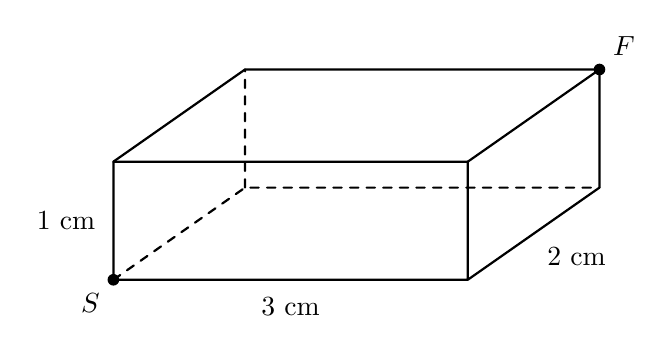
\begin{tikzpicture}[scale=1.5, line join=round, line cap=round]
\def\cuboidlength{3}
\def\cuboiddepth{2}
\def\cuboidheight{1}
\def\depthangle{35}
\pgfmathsetmacro{\projecteddepth}{0.68*\cuboiddepth}

% Projected cuboid vertices
\coordinate (S) at (0,0);
\coordinate (B) at (\cuboidlength,0);
\coordinate (D) at ($(S)+(\depthangle:\projecteddepth)$);
\coordinate (C) at ($(B)+(\depthangle:\projecteddepth)$);
\coordinate (A) at ($(S)+(0,\cuboidheight)$);
\coordinate (E) at ($(B)+(0,\cuboidheight)$);
\coordinate (H) at ($(D)+(0,\cuboidheight)$);
\coordinate (F) at ($(C)+(0,\cuboidheight)$);

% Hidden edges
\draw[thick, dashed, black] (S) -- (D) -- (C);
\draw[thick, dashed, black] (D) -- (H);

% Visible edges
\draw[thick, black] (S) -- (B) -- (E) -- (A) -- cycle;
\draw[thick, black] (B) -- (C) -- (F) -- (E);
\draw[thick, black] (A) -- (H) -- (F);

% Marked opposite corners
\fill[black] (S) circle (1.4pt);
\fill[black] (F) circle (1.4pt);

% Corner labels
\node[below left=2pt] at (S) {$S$};
\node[above right=2pt] at (F) {$F$};

% Edge-length labels
\path (S) -- (B) node[midway, below=3pt] {$3\text{ cm}$};
\path (B) -- (C) node[midway, below right=2pt] {$2\text{ cm}$};
\path (S) -- (A) node[midway, left=3pt] {$1\text{ cm}$};
\end{tikzpicture}
% end q000649 diagram
\end{center}

\par\vspace*{12pt}
\begin{tabularx}{\linewidth}{@{}>{\bfseries}l Y@{}}
A &
% begin q000649 choice A
$\sqrt{14}$ cm
% end q000649 choice A
\\[0.8em]
B &
% begin q000649 choice B
$3\sqrt{2}$ cm
% end q000649 choice B
\\[0.8em]
C &
% begin q000649 choice C
$2\sqrt{5}$ cm
% end q000649 choice C
\\[0.8em]
D &
% begin q000649 choice D
$1+\sqrt{13}$ cm
% end q000649 choice D
\\[0.8em]
E &
% begin q000649 choice E
$\sqrt{26}$ cm
% end q000649 choice E
\\[0.8em]
F &
% begin q000649 choice F
$6$ cm
% end q000649 choice F
\\
\end{tabularx}
\end{enumerate}
\clearpage
\thispagestyle{djspaper}
\vspace*{8pt}
\djsTopicLine{Integration}
\begin{enumerate}[label=\textbf{\arabic*.},leftmargin=*,itemsep=0pt,start=9]
\questionitem[Integration]
% begin q000156 stem
Let $\lfloor x\rfloor$ denote the greatest integer less than or equal to $x$.

Define \[ f(x)=\lfloor 2x\rfloor-\lfloor x\rfloor \] for all real $x$.

The value of $\displaystyle \int_0^2 f(x)\,\mathrm{d}x$ is
% end q000156 stem

\par\vspace*{12pt}
\begin{tabularx}{\linewidth}{@{}>{\bfseries}l Y@{}}
A &
% begin q000156 choice A
$0$
% end q000156 choice A
\\[0.8em]
B &
% begin q000156 choice B
$\dfrac{1}{2}$
% end q000156 choice B
\\[0.8em]
C &
% begin q000156 choice C
$1$
% end q000156 choice C
\\[0.8em]
D &
% begin q000156 choice D
$\dfrac{3}{2}$
% end q000156 choice D
\\[0.8em]
E &
% begin q000156 choice E
$2$
% end q000156 choice E
\\[0.8em]
F &
% begin q000156 choice F
$3$
% end q000156 choice F
\\[0.8em]
G &
% begin q000156 choice G
$4$
% end q000156 choice G
\\
\end{tabularx}
\end{enumerate}
\clearpage
\thispagestyle{djspaper}
\vspace*{8pt}
\djsTopicLine{Logic}
\begin{enumerate}[label=\textbf{\arabic*.},leftmargin=*,itemsep=0pt,start=10]
\questionitem[Logic]
% begin q000782 stem
Let $f$ be a polynomial defined for all real numbers $x$.

Let $g$ be the function defined by
\[
g(x) = \int_0^x f(t)\,\mathrm{d}t
\]
for all real numbers $x$.

Consider the following three conditions on $f$:
\[
\begin{array}{@{}ll@{}}
\textbf{1} & x f(x) \ge 0\text{ for all real numbers }x \\[5pt]
\textbf{2} & g(x) \ge 0\text{ for all real numbers }x \\[5pt]
\textbf{3} & f(0) = 0\\[5pt]
\end{array}
\]
Consider also the following three statements:
\[
\begin{array}{@{}ll@{}}
\textbf{I} & \text{Condition 1 is necessary for Condition 2} \\[5pt]
\textbf{II} & \text{Condition 1 is sufficient for Condition 2} \\[5pt]
\textbf{III} & \text{Condition 3 is necessary for Condition 2} \\[5pt]
\end{array}
\]
Which of the statements I, II and III is/are true?
% end q000782 stem

\par\vspace*{12pt}
\begin{tabularx}{\linewidth}{@{}>{\bfseries}l Y@{}}
A &
% begin q000782 choice A
None of them
% end q000782 choice A
\\[0.8em]
B &
% begin q000782 choice B
I only
% end q000782 choice B
\\[0.8em]
C &
% begin q000782 choice C
II only
% end q000782 choice C
\\[0.8em]
D &
% begin q000782 choice D
III only
% end q000782 choice D
\\[0.8em]
E &
% begin q000782 choice E
I and II only
% end q000782 choice E
\\[0.8em]
F &
% begin q000782 choice F
I and III only
% end q000782 choice F
\\[0.8em]
G &
% begin q000782 choice G
II and III only
% end q000782 choice G
\\[0.8em]
H &
% begin q000782 choice H
I, II and III
% end q000782 choice H
\\
\end{tabularx}
\end{enumerate}
\clearpage
\thispagestyle{djspaper}
\vspace*{8pt}
\djsTopicLine{Number}
\begin{enumerate}[label=\textbf{\arabic*.},leftmargin=*,itemsep=0pt,start=11]
\questionitem[Number]
% begin q000734 stem
Let $N=2^8\times3^6$ 

A positive integer $k$ is called \textit{suitable} if both $\dfrac{N}{k^2}$ and $\dfrac{k^3}{N}$ are integers. 

What is the sum of all suitable values of $k$?
% end q000734 stem

\par\vspace*{12pt}
\begin{tabularx}{\linewidth}{@{}>{\bfseries}l Y@{}}
A &
% begin q000734 choice A
$432$
% end q000734 choice A
\\[0.8em]
B &
% begin q000734 choice B
$576$
% end q000734 choice B
\\[0.8em]
C &
% begin q000734 choice C
$648$
% end q000734 choice C
\\[0.8em]
D &
% begin q000734 choice D
$864$
% end q000734 choice D
\\[0.8em]
E &
% begin q000734 choice E
$1296$
% end q000734 choice E
\\
\end{tabularx}
\end{enumerate}
\clearpage
\thispagestyle{djspaper}
\vspace*{8pt}
\djsTopicLine{Proof \& Error Analysis}
\begin{enumerate}[label=\textbf{\arabic*.},leftmargin=*,itemsep=0pt,start=12]
\questionitem[Proof \& Error Analysis]
% begin q000786 stem
In this question you may use the facts \[\sin\dfrac{\pi}{12}=\dfrac{\sqrt{6}-\sqrt{2}}{4} \qquad\text{and}\qquad\sin\dfrac{5\pi}{12}=\dfrac{\sqrt{6}+\sqrt{2}}{4}\] \vspace*{5pt}


A student attempts to answer the following question.

\begin{center}
\begin{minipage}{0.82\linewidth}
\centering
Find all real values of $x$, with $0<x<\pi$, such that $\log_{2}(\sin x)+\log_{2}(\cos x)=-2$.
\end{minipage}
\end{center}

The student's attempt is as follows.

\[
\begin{array}{@{}ll@{}}
\textbf{I} & \text{Using the laws of logarithms, the equation becomes } \log_{2}(\sin x\cos x)=-2 \\[10pt]
\textbf{II} & \text{Hence } \sin x\cos x=\dfrac{1}{4} \\[10pt]
\textbf{III} & \text{Every solution must therefore satisfy } \sin^{2}x\cos^{2}x=\dfrac{1}{16} \\[10pt]
\textbf{IV} & \text{Writing}\ \cos^{2}x=1-\sin^{2}x\ \text{and}\ s=\sin^{2}x\text{ this becomes } 16s^{2}-16s+1=0 \\[10pt]
\textbf{V} & \text{Hence every solution must have } s=\dfrac{2\pm\sqrt{3}}{4}\text{, and since}\\[8pt]& \sin x>0\ \text{for}\ 0<x<\pi\text{,}\, \sin x=\dfrac{\sqrt{6}\pm\sqrt{2}}{4} \\[10pt]
\textbf{VI} & \text{Therefore } x=\dfrac{\pi}{12},\ \dfrac{5\pi}{12},\ \dfrac{7\pi}{12},\dfrac{11\pi}{12} \\[10pt]
\end{array}
\]

Which of the following best describes the attempt?
% end q000786 stem

\par\vspace*{12pt}
\begin{tabularx}{\linewidth}{@{}>{\bfseries}l Y@{}}
A &
% begin q000786 choice A
The attempt is completely correct.
% end q000786 choice A
\\[0.8em]
B &
% begin q000786 choice B
The attempt is incorrect, and the first error occurs in line I.
% end q000786 choice B
\\[0.8em]
C &
% begin q000786 choice C
The attempt is incorrect, and the first error occurs in line III.
% end q000786 choice C
\\[0.8em]
D &
% begin q000786 choice D
The attempt is incorrect, and the first error occurs in line IV.
% end q000786 choice D
\\[0.8em]
E &
% begin q000786 choice E
The attempt is incorrect, and the first error occurs in line V.
% end q000786 choice E
\\[0.8em]
F &
% begin q000786 choice F
The attempt is incorrect, and the first error occurs in line VI.
% end q000786 choice F
\\
\end{tabularx}
\end{enumerate}
\clearpage
\thispagestyle{djspaper}
\vspace*{8pt}
\djsTopicLine{Number}
\begin{enumerate}[label=\textbf{\arabic*.},leftmargin=*,itemsep=0pt,start=13]
\questionitem[Number]
% begin q000730 stem
There is a non-negative integer $k$ such that the binomial coefficient $\dbinom{64}{32}$ is divisible by $2^k$ but not by $2^{k+1}$ 

What is the value of $k$?
% end q000730 stem

\par\vspace*{12pt}
\begin{tabularx}{\linewidth}{@{}>{\bfseries}l Y@{}}
A &
% begin q000730 choice A
$0$
% end q000730 choice A
\\[0.8em]
B &
% begin q000730 choice B
$1$
% end q000730 choice B
\\[0.8em]
C &
% begin q000730 choice C
$2$
% end q000730 choice C
\\[0.8em]
D &
% begin q000730 choice D
$16$
% end q000730 choice D
\\[0.8em]
E &
% begin q000730 choice E
$31$
% end q000730 choice E
\\[0.8em]
F &
% begin q000730 choice F
$32$
% end q000730 choice F
\\[0.8em]
G &
% begin q000730 choice G
$63$
% end q000730 choice G
\\
\end{tabularx}
\end{enumerate}
\clearpage
\thispagestyle{djspaper}
\vspace*{8pt}
\djsTopicLine{Probability \& Counting}
\begin{enumerate}[label=\textbf{\arabic*.},leftmargin=*,itemsep=0pt,start=14]
\questionitem[Probability \& Counting]
% begin q000781 stem
Two cards are drawn in order, without replacement, from cards numbered $1$ to $6$. 

Consider the events
\[
\begin{array}{@{}ll@{}}
\textbf{A} & \text{The first card has an even number} \\[5pt]
\textbf{B} & \text{The second card has an even number} \\[5pt]
\textbf{C} & \text{The sum of the two numbers is odd} \\[5pt]
\end{array}
\]

We say that two events are \emph{independent} if the probability that both occur is equal to their individual probabilities multiplied together.

In notation, \[A \text{ and } B \text{ are independent} \quad\iff\quad P(A \text{ and } B) = P(A)\times P(B)\]

Which pairs of the events $A, B$ and $C$ are independent?
% end q000781 stem

\par\vspace*{12pt}
\begin{tabularx}{\linewidth}{@{}>{\bfseries}l Y@{}}
A &
% begin q000781 choice A
None of the three pairs
% end q000781 choice A
\\[0.8em]
B &
% begin q000781 choice B
$A$ and $B$ only
% end q000781 choice B
\\[0.8em]
C &
% begin q000781 choice C
$A$ and $C$ only
% end q000781 choice C
\\[0.8em]
D &
% begin q000781 choice D
$B$ and $C$ only
% end q000781 choice D
\\[0.8em]
E &
% begin q000781 choice E
$A$ and $C$; $B$ and $C$
% end q000781 choice E
\\
\end{tabularx}
\end{enumerate}
\clearpage
\thispagestyle{djspaper}
\vspace*{8pt}
\djsTopicLine{Probability \& Counting}
\begin{enumerate}[label=\textbf{\arabic*.},leftmargin=*,itemsep=0pt,start=15]
\questionitem[Probability \& Counting]
% begin q000780 stem
A positive integer is called \emph{ascending} if it has at least two digits and, reading its digits from left to right, each digit is strictly greater than the one before it. 

For example, $259$ is ascending, but $2556$ and $92$ are not.

How many ascending integers are there less than $10000$?
% end q000780 stem

\par\vspace*{12pt}
\begin{tabularx}{\linewidth}{@{}>{\bfseries}l Y@{}}
A &
% begin q000780 choice A
$126$
% end q000780 choice A
\\[0.8em]
B &
% begin q000780 choice B
$210$
% end q000780 choice B
\\[0.8em]
C &
% begin q000780 choice C
$246$
% end q000780 choice C
\\[0.8em]
D &
% begin q000780 choice D
$255$
% end q000780 choice D
\\[0.8em]
E &
% begin q000780 choice E
$375$
% end q000780 choice E
\\[0.8em]
F &
% begin q000780 choice F
$495$
% end q000780 choice F
\\[0.8em]
G &
% begin q000780 choice G
$3600$
% end q000780 choice G
\\
\end{tabularx}
\end{enumerate}
\clearpage
\thispagestyle{djspaper}
\vspace*{8pt}
\djsTopicLine{Number}
\begin{enumerate}[label=\textbf{\arabic*.},leftmargin=*,itemsep=0pt,start=16]
\questionitem[Number]
% begin q000007 stem
Let $n$ be a positive integer. Consider the following conditions: \[ \begin{array}{@{}l l@{}}
\textbf{I:} & \text{$n$ is even} \\[2pt]
\textbf{II:} & \text{$n$ is a multiple of $3$} \\[2pt]
\textbf{III:} & \text{$n$ is a prime greater than $3$}
\end{array} \] Which of these conditions is/are \textbf{sufficient} for the statement: \[2^n-1 \text{ is divisible by }7\]
% end q000007 stem

\par\vspace*{12pt}
\begin{tabularx}{\linewidth}{@{}>{\bfseries}l Y@{}}
A &
% begin q000007 choice A
I only
% end q000007 choice A
\\[0.8em]
B &
% begin q000007 choice B
II only
% end q000007 choice B
\\[0.8em]
C &
% begin q000007 choice C
III only
% end q000007 choice C
\\[0.8em]
D &
% begin q000007 choice D
I and II only
% end q000007 choice D
\\[0.8em]
E &
% begin q000007 choice E
I and III only
% end q000007 choice E
\\[0.8em]
F &
% begin q000007 choice F
II and III only
% end q000007 choice F
\\[0.8em]
G &
% begin q000007 choice G
I, II, and III
% end q000007 choice G
\\[0.8em]
H &
% begin q000007 choice H
None of them
% end q000007 choice H
\\
\end{tabularx}
\end{enumerate}
\clearpage
\thispagestyle{djspaper}
\vspace*{8pt}
\djsTopicLine{Proof \& Error Analysis}
\begin{enumerate}[label=\textbf{\arabic*.},leftmargin=*,itemsep=0pt,start=17]
\questionitem[Proof \& Error Analysis]
% begin q000151 stem
A statement is given: \[\text{S: For all real numbers $x$, \textbf{if} $x^2 \ge 1$ \textbf{then} $x^4 \ge x^2$}\] A student wishes to prove $S$ by contradiction and writes the following argument:

Assume that there exists a real number $x$ such that $x^2 \ge 1$ \textbf{and} $x^4 < x^2$ \[ \begin{array}{@{}l l@{}}
\textbf{I:} & \text{Then $x^4 - x^2 < 0$} \\[5pt]
\textbf{II:} & \text{So $x^2(x^2 - 1) < 0$} \\[5pt]
\textbf{III:} & \text{So $x^2 - 1 < 0$} \\[5pt]
\textbf{IV:} & \text{So $x^2 < 1$, which contradicts $x^2 \ge 1$}
\end{array} \] Therefore the original statement $S$ is concluded to be true.

Which of the following best describes this argument?
% end q000151 stem

\par\vspace*{12pt}
\begin{tabularx}{\linewidth}{@{}>{\bfseries}l Y@{}}
A &
% begin q000151 choice A
It is completely correct.
% end q000151 choice A
\\[0.8em]
B &
% begin q000151 choice B
It is incorrect, but it would be correct if written in the reverse order.
% end q000151 choice B
\\[0.8em]
C &
% begin q000151 choice C
It is incorrect, and the student has actually shown that $S$ is false.
% end q000151 choice C
\\[0.8em]
D &
% begin q000151 choice D
It is incorrect because line \textbf{II} does not follow from line \textbf{I}.
% end q000151 choice D
\\[0.8em]
E &
% begin q000151 choice E
It is incorrect because line \textbf{III} does not follow from line \textbf{II}.
% end q000151 choice E
\\[0.8em]
F &
% begin q000151 choice F
It is incorrect because the student has not really used proof by contradiction.
% end q000151 choice F
\\
\end{tabularx}
\end{enumerate}
\clearpage
\thispagestyle{djspaper}
\vspace*{8pt}
\djsTopicLine{Integration}
\begin{enumerate}[label=\textbf{\arabic*.},leftmargin=*,itemsep=0pt,start=18]
\questionitem[Integration]
% begin q000622 stem
The region $R$ in the first quadrant is bounded by the curve $y = 4x - x^2$ and the $x$-axis.

The line $y = 2x$ divides $R$ into two sub-regions: $R_1$, which lies above the line, and $R_2$, which lies below the line.

What is the ratio of the area of $R_1$ to the area of $R_2$?
% end q000622 stem

\begin{center}
% begin q000622 diagram
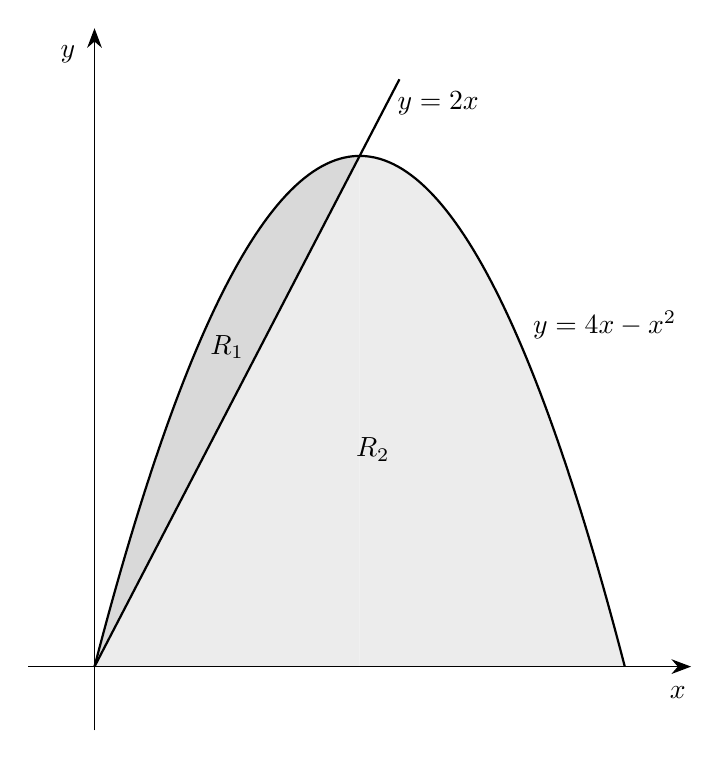
\begin{tikzpicture}
\pgfplotsset{compat=1.18}
\begin{axis}[
    width=10cm,
    height=10.5cm,
    xmin=-0.5, xmax=4.5,
    ymin=-0.5, ymax=5,
    axis lines=middle,
    axis line style={-{Stealth[length=2.5mm]}},
    axis on top,
    xtick=\empty,
    ytick=\empty,
    clip=true,
    samples=120
]
% Exact paths used to shade R_1.
\addplot[draw=none, name path=rOneCurve, domain=0:2]
    {4*x-x^2};
\addplot[draw=none, name path=rOneLine, domain=0:2, samples=2]
    {2*x};
\addplot[gray!30, draw=none]
    fill between[of=rOneCurve and rOneLine];

% Exact component paths used to shade R_2.
\addplot[draw=none, name path=rTwoLine, domain=0:2, samples=2]
    {2*x};
\addplot[draw=none, name path=rTwoAxisA, domain=0:2, samples=2]
    {0};
\addplot[gray!15, draw=none]
    fill between[of=rTwoLine and rTwoAxisA];

\addplot[draw=none, name path=rTwoCurve, domain=2:4]
    {4*x-x^2};
\addplot[draw=none, name path=rTwoAxisB, domain=2:4, samples=2]
    {0};
\addplot[gray!15, draw=none]
    fill between[of=rTwoCurve and rTwoAxisB];

% Boundary curve and dividing line.
\addplot[thick, black, domain=0:4]
    {4*x-x^2}
    node[pos=0.72, above right] {$y=4x-x^2$};
\addplot[thick, black, domain=0:2.3, samples=2]
    {2*x}
    node[pos=0.96, right] {$y=2x$};

% Region and axis labels.
\node at (axis cs:1,2.5) {$R_1$};
\node at (axis cs:2.1,1.7) {$R_2$};
\node at (axis cs:4.4,-0.2) {$x$};
\node at (axis cs:-0.2,4.8) {$y$};
\end{axis}
\end{tikzpicture}
% end q000622 diagram
\end{center}

\par\vspace*{12pt}
\begin{tabularx}{\linewidth}{@{}>{\bfseries}l Y@{}}
A &
% begin q000622 choice A
$1 : 3$
% end q000622 choice A
\\[0.8em]
B &
% begin q000622 choice B
$1 : 4$
% end q000622 choice B
\\[0.8em]
C &
% begin q000622 choice C
$1 : 7$
% end q000622 choice C
\\[0.8em]
D &
% begin q000622 choice D
$1 : 8$
% end q000622 choice D
\\[0.8em]
E &
% begin q000622 choice E
$1 : 15$
% end q000622 choice E
\\
\end{tabularx}
\end{enumerate}
\clearpage
\thispagestyle{djspaper}
\vspace*{8pt}
\djsTopicLine{Exponentials \& Logarithms}
\begin{enumerate}[label=\textbf{\arabic*.},leftmargin=*,itemsep=0pt,start=19]
\questionitem[Exponentials \& Logarithms]
% begin q000728 stem
The curve $C$ has equation
\[\log_2(2y+4)=2\log_2(x+1)\]

For which values of the real constant $m$ does the line $y=mx$ meet $C$ at exactly two distinct points?
% end q000728 stem

\par\vspace*{12pt}
\begin{tabularx}{\linewidth}{@{}>{\bfseries}l Y@{}}
A &
% begin q000728 choice A
$m<2$
% end q000728 choice A
\\[0.8em]
B &
% begin q000728 choice B
$m\le 2$
% end q000728 choice B
\\[0.8em]
C &
% begin q000728 choice C
$m>0$
% end q000728 choice C
\\[0.8em]
D &
% begin q000728 choice D
$m>2$
% end q000728 choice D
\\[0.8em]
E &
% begin q000728 choice E
$m\ge 2$
% end q000728 choice E
\\
\end{tabularx}
\end{enumerate}
\clearpage
\thispagestyle{djspaper}
\vspace*{8pt}
\djsTopicLine{Logic}
\begin{enumerate}[label=\textbf{\arabic*.},leftmargin=*,itemsep=0pt,start=20]
\questionitem[Logic]
% begin q000784 stem
For a real constant $a$, the function $f$ is defined for $x>0$ by $f(x)=\sqrt{x}+\dfrac{a}{\sqrt{x}}$

Consider the conditions
\[
\begin{array}{@{}ll@{}}
\textbf{I} & f'(4)>0 \\[5pt]
\textbf{II} & f(4)>f(1) \\[5pt]
\end{array}
\]

Which of the following describes the relationship between conditions I and II?
% end q000784 stem

\par\vspace*{12pt}
\begin{tabularx}{\linewidth}{@{}>{\bfseries}l Y@{}}
A &
% begin q000784 choice A
I is necessary but not sufficient for II.
% end q000784 choice A
\\[0.8em]
B &
% begin q000784 choice B
I is sufficient but not necessary for II.
% end q000784 choice B
\\[0.8em]
C &
% begin q000784 choice C
I is both necessary and sufficient for II.
% end q000784 choice C
\\[0.8em]
D &
% begin q000784 choice D
I is neither necessary nor sufficient for II.
% end q000784 choice D
\\[0.8em]
E &
% begin q000784 choice E
I and II cannot both be true.
% end q000784 choice E
\\
\end{tabularx}
\end{enumerate}
\end{document}
